\section{Methodologies and Experiments}
\begin{figure}
    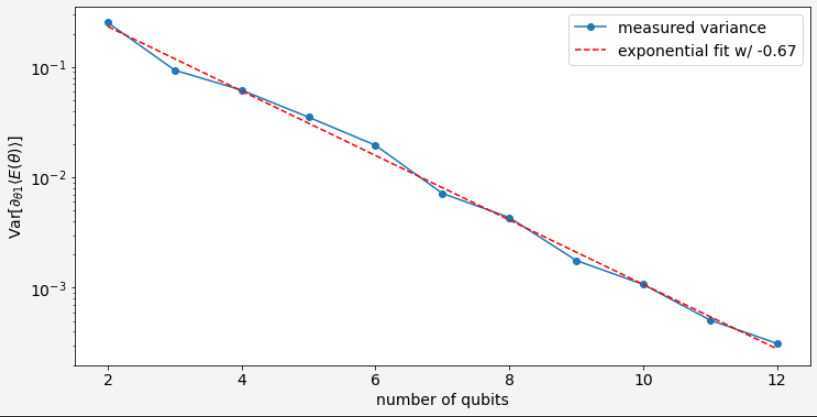
\includegraphics[width=\textwidth]{./ResearchDesign/Appendices/VarianceShrinking.png}
    \caption{
        An example of the Barren Plateaus phenomenon occurs in a QNN model. 
        The variance of the gradient shrinks \textit{exponentially} with the number of qubits. 
        Barren Plateaus phenomenon prevents optimisation algorithms from navigating the cost function landscape efficiently.
    }
    \label{Variance Shrinking demo}
\end{figure}



Cerezo et al. has pointed out that Barren Plateaus are cost function dependent \cite{cerezoCostFunctionDependent2021}, implying that the only way to eliminate Barren Plateaus fully is to use a local cost function with a shallow circuit.
However, other approaches can still mitigate the phenomenon without using the local cost function.
Skolik et al. and Liu et al. \cite{skolikLayerwiseLearningQuantum2021, liuParameterInitializationMethod2021} suggest that we can initiate the starting parameters away from plateaus to guarantee the trainability from the first steps.
In this section, we design the methodologies to conduct the experiment to answer the research question.

\subsection{Research Type Overview}
We have examined the three theories \cite{cerezoCostFunctionDependent2021, liuParameterInitializationMethod2021, skolikLayerwiseLearningQuantum2021} in the literature review, and it is suggested that an empirical experiment can be conducted to compare the three.
Consequently, the result of this experiment is a table that records the performance of the three methods in some criteria.

The main advantage of experimentation methodology is that we can fully control the experiment environment and its subjects, objects, etc.
In this case, these are the factors that lead to Barren Plateaus, the configuration for the QNN ansatz, and the three implementations of theories on the QNN ansatz.
We elaborate on the research process in later sections.

\begin{figure}
    \centering
    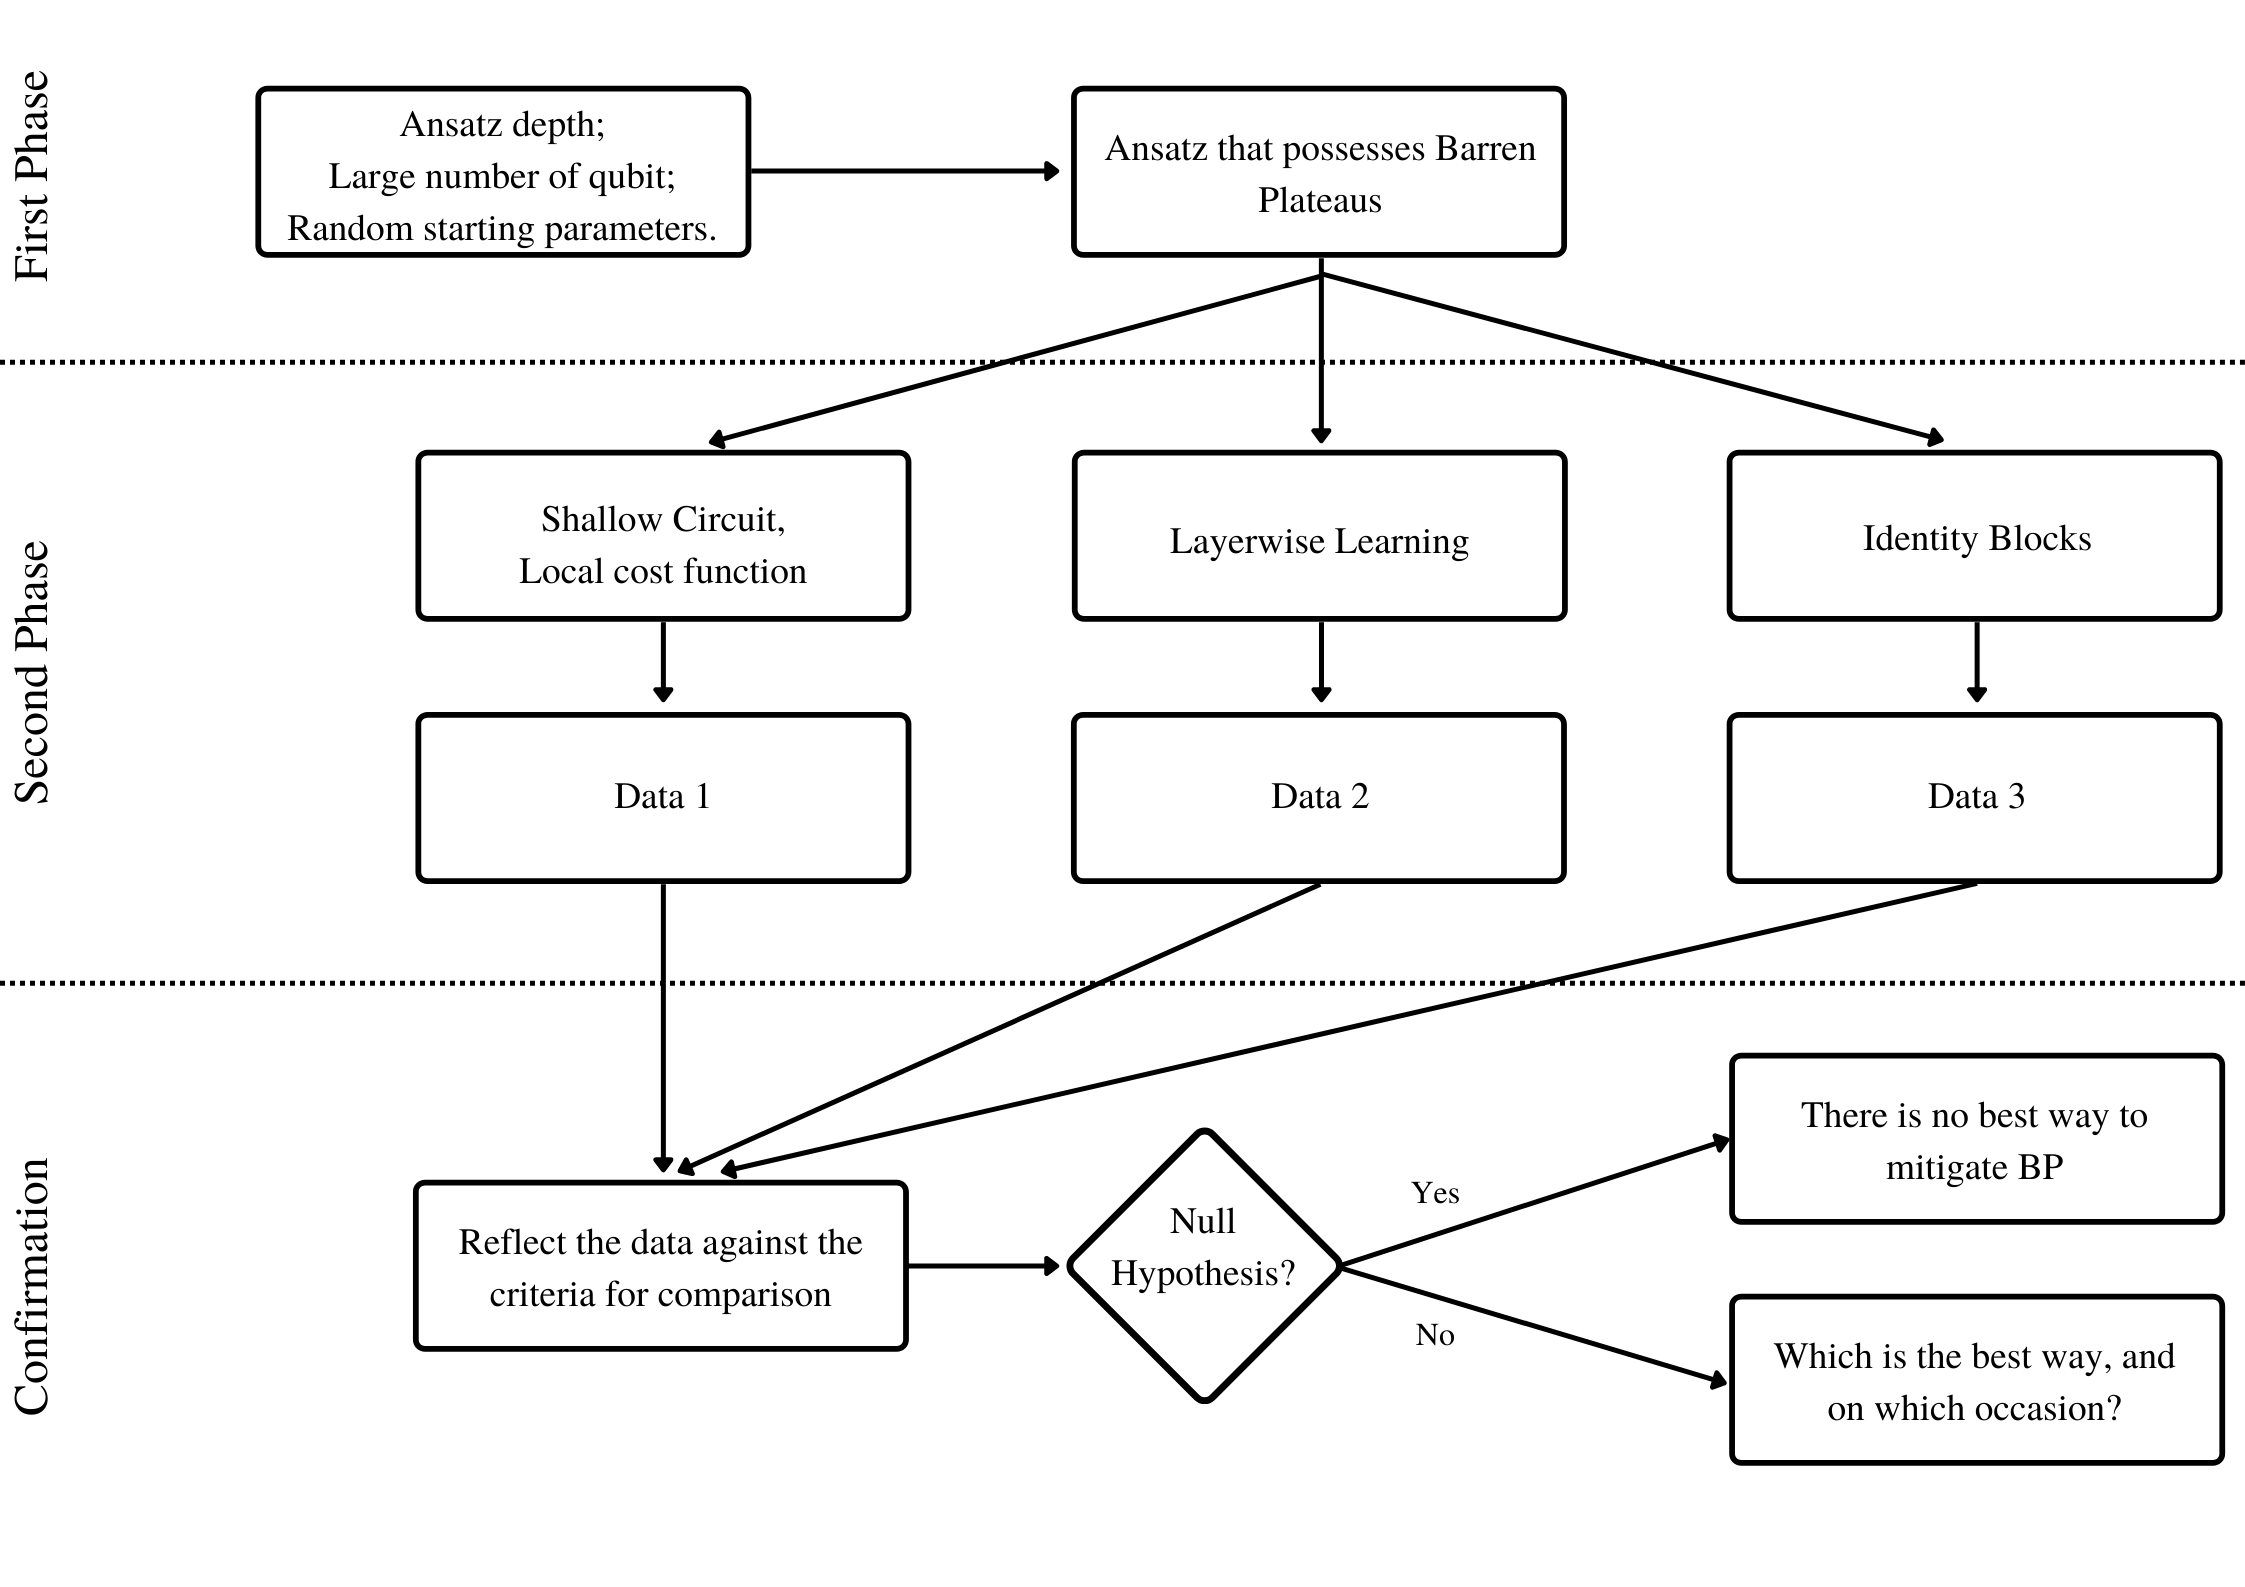
\includegraphics[width=\textwidth]{./ResearchDesign/Appendices/Method.png}
    \caption{
        Research method in summary.
    }
    \label{Research Activities}
\end{figure}

\subsection{Research Activities}
\label{Research Activities section}
\textbf{In the first phase, we create a QNN model to reproduce the Barren Plateaus.} 
We can use Qiskit \cite{Qiskit} to construct the ansatz, and most importantly, it provides a quantum emulator capable of simulating up to 32 qubits.
The literature review had pointed out that the two factors causing Barren Plateaus are the \textit{ansatz depth, a large number of qubits} and the \textit{randomised starting parameters}, so we configure the ansatz to have such characteristics in a quantum simulator.
Then we calculate the gradient variance and expect the variance to shrink \textit{exponentially} with the number of qubits (see Figure \ref{Variance Shrinking demo}).
The result will be a QNN ansatz with the depth and number of qubits enough to produce the Barren Plateaus.

\textbf{In the second phase, we implement the three approaches}.
With the QNN ansatz from the first step, we can implement the three methods discussed in the literature review.
The Qiskit framework also supports the mutation for the ansatz object, such as the number of qubits to measure, the depth of ansatz (repetition) and the starting parameters.
We will track the variances of the gradient for each method to identify if the model has mitigated the Barren Plateaus phenomenon.

The results of the research activities are discussed in the Subsection \ref{Data Collecting Section}.

\subsubsection{Criteria}
\label{Criteria section}
We can compare the data with these criteria:
\begin{itemize}
    \item How good the solution is;
    \item The size of the circuit;
    \item The size of the qubit registry;
    \item The time required to execute the circuit;
    \item The complexity of the algorithms.
\end{itemize}

\subsubsection{Hypothesis}
The experiment activities are formalised into two hypotheses:
\begin{itemize}
    \item \textbf{Null}: The three methods have the same performance according to the criteria, or the difference is insignificant;
    \item \textbf{Alternative}: The three methods' performance differs when reflecting the result against the criteria.
\end{itemize}

\subsection{Data Collecting Method}
\label{Data Collecting Section}
Here we discuss our method to collect the data from the experiment.

The output of the first phase is a Qiskit ansatz object that contains the number of qubits, the depth of the circuit (rep), and the parameter configured randomly.
Moreover, the ansatz object in Qiskit is mutable, which means we can modify the ansatz properties in the second phase.

For the second phase, we need to record three different outputs of the three methods accordingly, with the criteria defined in Subsection \ref{Criteria section}.
The result is a table with the rows of criteria in the Subsection \ref{Criteria section} with each method as rows.
With this data, we can decide whether to reject the null hypothesis or not.

Finally, we summarise the table to present the findings.

\subsection{Resources}
Most of our required resources are open-sources:
\begin{itemize}
    \item Python 3.6+: \url{https://www.python.org/downloads/}
    \item Anaconda: \url{https://www.anaconda.com/products/distribution}
    \item Jupyter Notebook: \url{https://jupyter.org/}
    \item Qiskit: \url{https://qiskit.org/}
    \item IBM Quantum: \url{https://quantum-computing.ibm.com/}
\end{itemize}

To prepare the quantum emulator on local machine, we first install Python and Anaconda for programming language support, Jupyter Notebook as a code editing tool.
Then we follow the official instruction from Qiskit \cite{Qiskit} to install the necessary packages.
We can start working with Qiskit in a Jupyter Notebook file.

The other option is to use the provided Python kernel with Qiskit pre-installed provided by IBM Quantum. 
While this is a convenient choice for online presentation or remote working because of instant access, this server has shortcomings, such as the maximum ram for open access is only 8 Gigabytes and the processing power is limited.

To construct the ansatz as discussed in Section \ref{Research Activities section}, we can use the "Real Amplitudes" circuit provided by Qiskit.


\subsection{Success Condition}
The experiment will be concluded when these conditions are met:
\begin{itemize}
    \item We have a QNN ansatz that possesses Barren Plateaus;
    \item The three methods are implemented;
    \item The data from the three methods are evaluated against the criteria;
    \item We have identified when to use which method to counter Barren Plateaus.
\end{itemize}